
\chapter{Evaluation of SHAMPU}
In order to assess the capabilities of SHAMPU, we planed and ran experiments designed to evaluate the SHAMPU framework according to the following use-cases:
\begin{itemize}
	\item{\textbf{Scheduled data-transmission}} \hfill \\ In order for SHAMPU to work as a debugging and logging platform, the base station needs to periodically receive data from all the nodes in the network. Furthermore the base station has to be able to send commands to nodes in the network.
	
	\item{\textbf{Unscheduled data-transmission}} \hfill \\ There are several cases, where it is not feasible to use a scheduled data-transmission. Because either the data only needs to be transmitted once, or it is not known at what point in time the transmission happens: 
	\begin{itemize}
		\item{}Reprogramming of a node: SHAMPU is able to reprogram the attached node. For this process, SHAMPU needs to receive a new firmware, which can amount to several hundred kB.
		\item{}SHAMPU RAM-Dumps: SHAMPU has 128kB of RAM, which can be used to save collected data during an experiment. At the end of the experiment the complete memory needs to be transmitted back to the base station.
	\end{itemize}
\end{itemize}
	
To evaluate ANT according to these two use-cases, we identified three metrics which indicate how well a use-case can be handled:
	\begin{itemize}
		\item {\textbf{Data throughput }} \hfill \\ The speed, with which ANT can transmit data, directly affects the network performance and how many nodes can be part of the network at the same time. ANT provides three different data types which can be used to transport data: Broadcast data and acknowledge data is typically used for scheduled data-transmission, whereas burst mode is used mostly for unscheduled data-transmission. 		
		
		\item {\textbf{Message delay}} \hfill \\ A SHAMPU base station not only acts as a data sink for incoming logging information, but is also able to send commands to other SHAMPU devices in the network.
		It is thus important to know how long it takes ANT to verify whether a message was correctly received or not.
		
		\item {\textbf{Communication range}} \hfill \\ Since SHAMPU is architecture independent it can be used in different situations. Therefore it is important to know, how far away from the base station the nodes can be placed. As SHAMPU focuses on energy efficiency, it might also be viable to reduce the range for smaller setups to save even more energy.
	\end{itemize}

To cover the mentioned metrics we designed different experiments, which test one or more of the described categories. The following section describes the experiments according to the following template:

\begin{description}
	\item{\textbf{Description}} \hfill \\ A description of the experiment and the category being evaluated.
	\item{\textbf{Use-Case}} \hfill \\ The use-case which the experiment tries to test.
	\item{\textbf{Network topology and pseudo code}} \hfill \\ A diagram of the network topology in which the experiment is run and pseudo code which describes the program being run on the master and the slave. Missing values are default values and described in section \ref{sec:commonPara}.
	\item{\textbf{Testing methodology}} \hfill \\ A description how the experiment is performed.
	\item{\textbf{Result}} \hfill \\ The results of the experiment and any additional data collected during the experiment.
\end{description}

\newpage

\section{Common experiment parameters}
\label{sec:commonPara}
\begin{figure}[H]
	\centering
	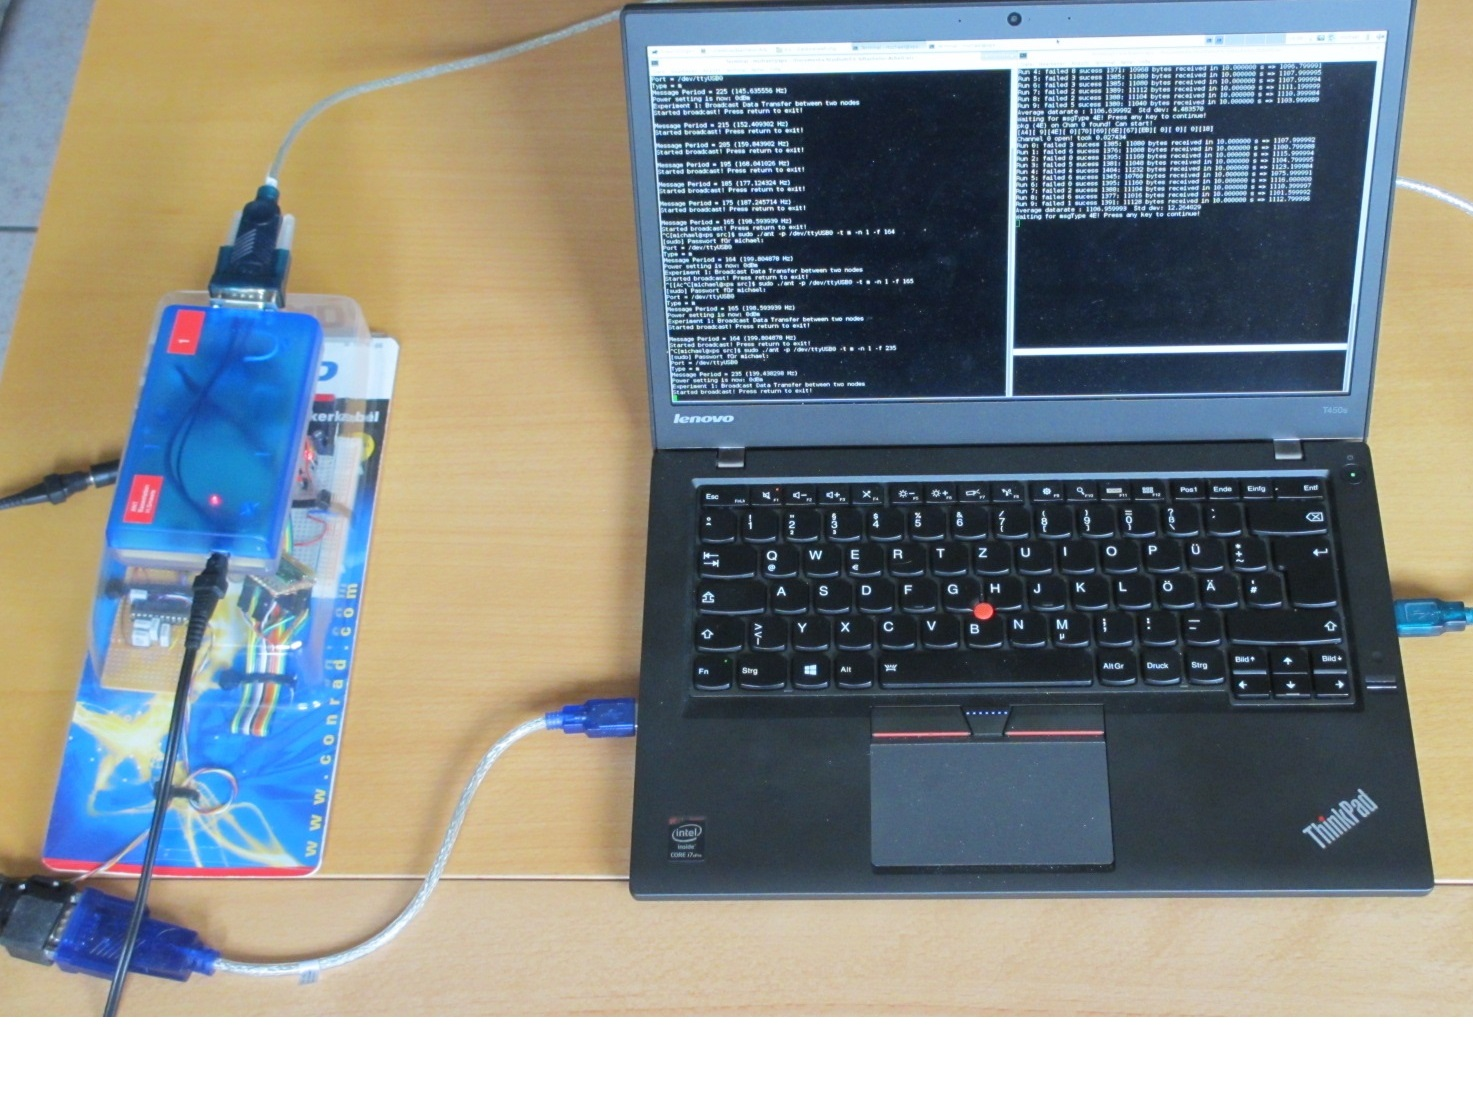
\includegraphics[scale=.5]{content/images/expSetup.JPG}
	\caption{Experiment setup}\label{fig:expSetup}
\end{figure}

If not otherwise noted in the description each experiment was run in the Mobility Lab of the Networked Embedded Systems group at the University of Duisburg-Essen (SA 327), with the two base stations in the configuration which can be seen in figure \ref{fig:expSetup}. The following table describes the parameters which were used in the experiments.

\begin{table}[H]
	\centering
	\begin{tabular}{|l|c|c|}
		\hline
		Device number        & 33    & \multirow{3}{*}{\begin{tabular}[c]{@{}c@{}}Channel ID\\ (see section \ref{sec:ANTchan})\end{tabular}}   \\ \cline{1-2}
		Device type          & 1     &                                                                                                         \\ \cline{1-2}
		Transmission type    & 1     &                                                                                                         \\ \hline
		ID\_CHAN1            & 0     & \multirow{2}{*}{\begin{tabular}[c]{@{}c@{}}Configuration\\ for the first channel\end{tabular}}          \\ \cline{1-2}
		FREQ\_CHAN1          & 66 Hz &                                                                                                         \\ \hline
		ID\_CHAN2            & 1     & \multirow{2}{*}{\begin{tabular}[c]{@{}c@{}}Configuration\\ for the second channel\end{tabular}}         \\ \cline{1-2}
		FREQ\_CHAN2          & 77 Hz &                                                                                                         \\ \hline
		STD\_FREQ            & 8192  & 4 Hz (default frequency)                                                                                \\ \hline
		min\_Channel\_Period & 165   & 198.6 Hz (closest to 200 Hz)                                                                            \\ \hline
		max\_Channel\_Period & 65535 & 0.5 Hz (smallest frequency)                                                                             \\ \hline
		STD\_POWER           & 0 dBm & 1 mW (default transmit power)                                                                           \\ \hline
	\end{tabular}
	\caption{ANT default configuration}
\end{table}

The channel period $p$ can be used to calculate the frequency of the messages $f_t = \frac{32678s^{-1}}{p}$. For example a message period of 8192 results in a message frequency of 4 Hz, which means that 4 messages are sent every second.

ANT supports different transmit power levels $x$: 0 dBm, -5 dBm, -10 dBm and -20 dBm. dBm is a way to express broadcast power as a power ratio in decibels. The power of the broadcast $p$ can be calculated as $p = 1mW * 10^{\frac{x}{10}}$.

Furthermore in experiments which measure data throughput, we show the maximum theoretical value for each frequency. This is the maximum value which can be achieved, if there are no transmission errors and no interference with other channels. The value depends on the message frequency $f$ and is calculated as $rate_{max}(f) = 8*f$. Each message contains a payload of 8 bytes and $f$ messages are sent each second.

The results for each experiment is always the average over all measured values. The displayed error margins are the standard deviation of all measured values. Additionally in some experiments we show the measured error rate, which is also averaged over all measured values.
\newpage

\section{Experiment 1: Broadcast Data Transfer between two nodes}
\begin{description} 
	\item{\textbf{Description}} \hfill \\ Broadcasting is one way of periodically transmitting data between two or more ANT nodes. Since all broadcast packets are synchronized to a fixed time slot, the data throughput can be increased by decreasing the channel period. The experiment itself is split into two parts. In the first part we try to determine the highest possible data throughput. Also we try to determine whether the channel period has an effect on the time it takes for a slave node to find and join an existing channel. The second part is a test of the highest detected data throughput. Here we try to evaluate if there are any variations of the data throughput over a much longer interval.	
	\item{\textbf{Use-Case}} \hfill \\ Scheduled data-transmission	
	\item{\textbf{Network topology and pseudo code}} \hfill \\ 
	\begin{figure}[H]
		\centering
		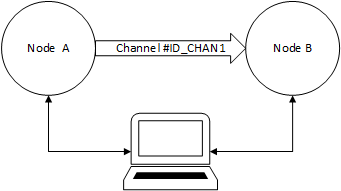
\includegraphics[scale=1]{content/images/exp_topo.png}
		\caption{Topology experiment 1}
	\end{figure}
	\begin{code}[H]
		\begin{verbatim}
		channelPeriod = max_Channel_Period
		while (channelPeriod >= min_Channel_Period)
		  ANT_SetChannelPeriod(ID_CHAN1, channelPeriod)
		  ANT_OpenChannel(ID_CHAN1, ANT_Bidirectional_Master)
		  ANT_SendBroadcastData(ID_CHAN1, [0x70, 0x69, 0x6E, 0x67])
		  wait_for_user_input()
		  ANT_CloseChannel(ID_CHAN1)
		  if (channelPeriod >= 0x00FF)
		    channelPeriod = channelPeriod >> 1
		  else
		    channelPeriod = channelPeriod - 10
		\end{verbatim}
		\caption{Broadcast data single channel (Master)}\label{lst:mExp1}
	\end{code}
	
	\begin{code}[H]
		\begin{verbatim}
		channelPeriod = max_Channel_Period
		while (channelPeriod >= min_Channel_Period) 
		  for (i in 0..10) 
		    ANT_SetChannelPeriod(ID_CHAN1, channelPeriod)
		    ANT_OpenChannel(ID_CHAN1, ANT_Bidirectional_Slave)
		    count = 0, fail = 0
		    for (100 seconds) 
		      if (receivedPacket() == ANT_BROADCAST_DATA)		        
		        count++;			  
		      else if (receivedPacket() == ANT_MESSAGE_EVENT_RX_FAIL)
		        fail++;
		    print (count * 8 / 100) + " Bytes per second"
		    print fail + " failed transmissions"
		    wait_for_user_input()
		    ANT_CloseChannel(ID_CHAN1)
		  if (channelPeriod >= 0x00FF)
		    channelPeriod = channelPeriod >> 1
		  else
		    channelPeriod = channelPeriod - 10
		\end{verbatim}
		\caption{Broadcast data single channel (Slave)}\label{lst:sExp1}
	\end{code}	
	\item{\textbf{Testing methodology}} \hfill \\Experiment 1 is split into two parts.
	In the first part node A acts as the master and node B as the slave. For both nodes the channel period is set to the highest value and the channel is opened. Node B records how long it takes to join the channel and how many bytes it receives over a 100s interval. The measurement is repeated 10 times and the average values are saved. Then the channel period is decreased and the process is repeated.\\ 
	In the second part of the experiment, the channel period is set to the value which achieved the highest speed. The experiment is then left running for a period of 10 hours and the data throughput is recorded in one continuous run.
	\item{\textbf{Result}} \hfill \\  
	\begin{figure}[H]
		\centering
		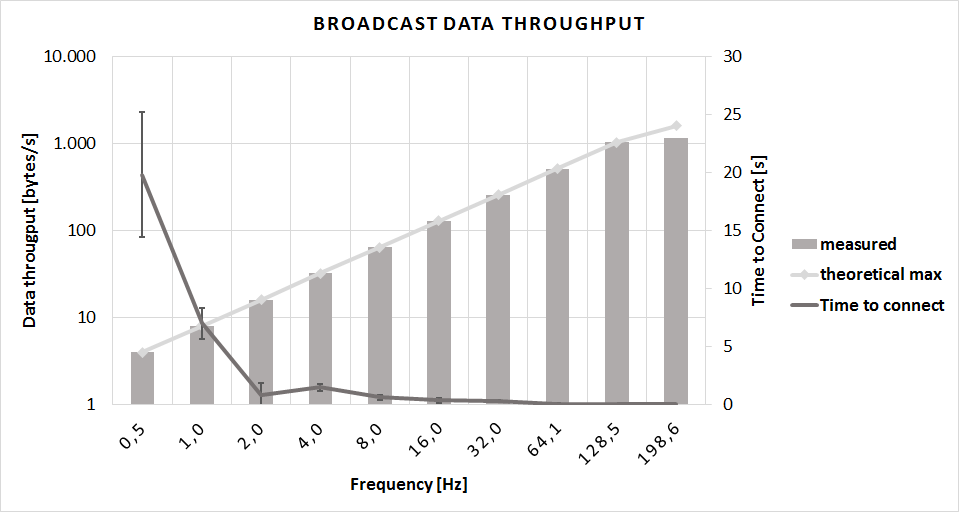
\includegraphics[scale=0.5]{content/images/exp1_norm.png}
		\caption{Broadcast data throughput (0.5Hz - 198.6Hz)}\label{fig:exp1norm}
	\end{figure}
	
	Figure \ref{fig:exp1norm} shows the transmission speeds achieved for the different frequencies. Up to a frequency of 128 Hz, the measured data throughput matches the expected theoretical maximum rate. For the highest measured frequency (198.6 Hz), the data throughput is lower than the maximum rate. The measured errors are insignificant. Therefore the frequencies between 128 Hz and 198.6 Hz were analyzed in more detail (see page \pageref{fig:exp1between}). 
		
	The time it takes for a node to join a channel is very short once the frequency is above 1 Hz. For frequencies above 64 Hz, the time it takes to join a channel becomes negligible, with times around 75 ms (see Figure \ref{fig:exp1norm}). All the measured values are below the specified worst case channel acquisition times of the ANT protocol \cite{AntChan}.
	
	\begin{figure}[H]
		\centering
		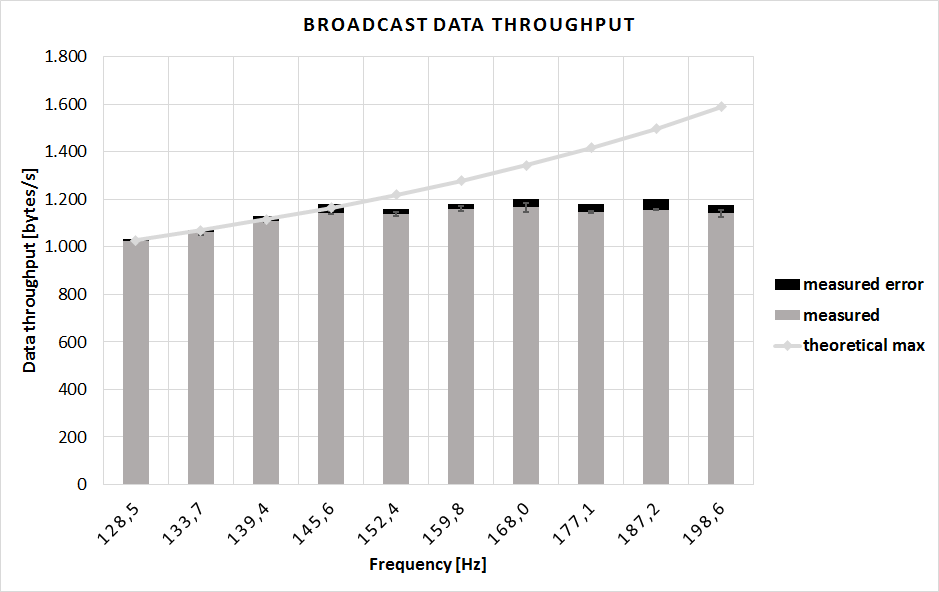
\includegraphics[scale=0.5]{content/images/exp1_detail.png}
		\caption{Broadcast data throughput (128.5Hz - 198.6Hz)}\label{fig:exp1between}
	\end{figure}
	As seen in figure \ref{fig:exp1between} the measured data throughputs for frequencies above 140 Hz all fall short of the maximum values. The average data throughput of these frequencies remains consistently at around 1100 Bps. The experiment was repeated multiple times, running it at different times and places, thus an environmental factor can be excluded. That means, the reason for the upper limit has to be found with the test setup itself. See section \ref{sec:dataThrougput} for a discussion about possible reasons for this upper limit.
	
	\begin{figure}[H]
		\centering
		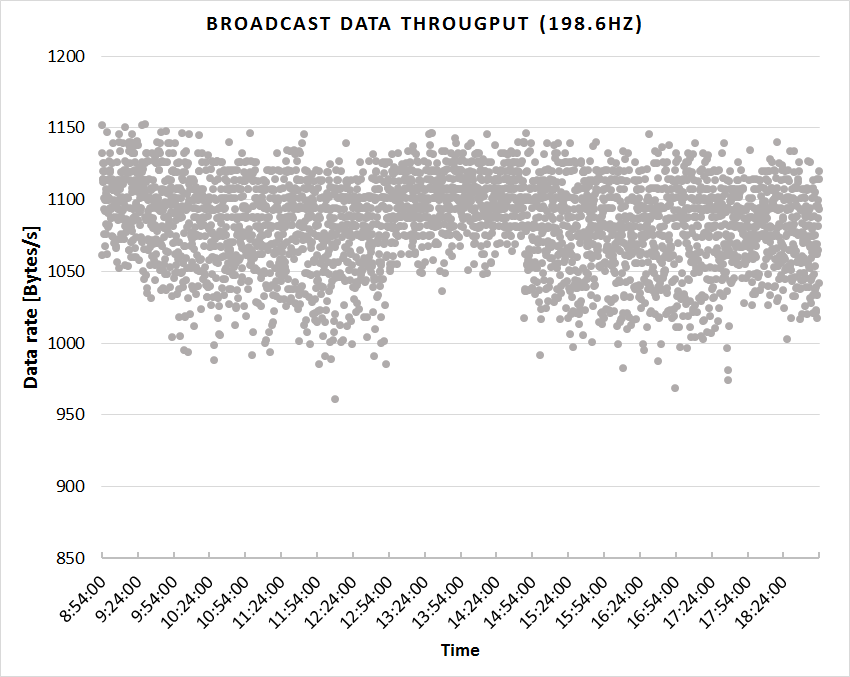
\includegraphics[scale=0.5]{content/images/exp1_long.png}
		\caption{Broadcast data throughput over time (198.6Hz)}\label{fig:exp1long}
	\end{figure}
	Figure \ref{fig:exp1long} shows the transmission speed for the highest supported frequency 198.6 Hz over time. The results show that the data throughput stays fairly consistent at around 1100 Bps with a standard deviation of only 30 Bps, or 2.7\%. Interesting to note is the time period from 1:00PM to 2:50 PM, where the deviation from the average is much smaller. The exact reason for this phenomenon in unknown, since during this time period the environment of the test setup did not change in any known way.
\end{description}
\newpage

\section{Experiment 2: Broadcast Data Transfer with two channels}
\begin{description} 
	\item{\textbf{Description}} \hfill \\ In experiment 1 we determined the channel period, which allows for the maximum throughput. In this experiment we try to determine, how the maximum throughput is affected by the number of channels in the network. SHAMPU needs two channels to work correctly: One channel which sends data from the base station to the nodes in order to control them, and another channel by which the nodes can send debugging and other information.
	\item{\textbf{Use-Case}} \hfill \\ Scheduled data-transmission	
	\item{\textbf{Network topology and pseudo code}} \hfill
	\begin{figure}[H]
		\centering
		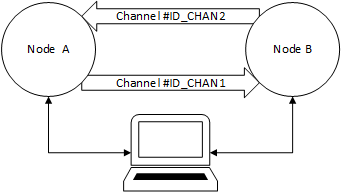
\includegraphics[scale=1]{content/images/exp2_topo.png}
		\caption{Topology experiment 2}
	\end{figure}
	\begin{code}[H]
		\begin{verbatim}
		channelPeriod = max_Channel_Period
		while (channelPeriod >= min_Channel_Period) 
		  ANT_SetChannelPeriod(ID_CHAN1, channelPeriod)
		  openChannel(ID_CHAN1, ANT_Bidirectional_Master)
		  ANT_SendBroadcastData(ID_CHAN1, [0x70, 0x69, 0x6E, 0x67])
		  ANT_SetChannelPeriod(ID_CHAN2, channelPeriod)
		  openChannel(ID_CHAN2, ANT_Bidirectional_Slave)
		  count = 0
		  for (100 seconds) 
		    if (receivedPacket() == ANT_BROADCAST_DATA)
		      count++			
		  print (count * 8 / 100) + " Bytes per second"
		  wait_for_user_input()
		  ANT_CloseChannel(ID_CHAN1)
		  ANT_CloseChannel(ID_CHAN2)
		  if (channelPeriod >= 0x01FF)
		    channelPeriod = channelPeriod >> 1
		  else
		    channelPeriod = channelPeriod - 10
		 \end{verbatim}
		\caption{Broadcast data transfer two channels (Master)}\label{lst:mExp2}
	\end{code}
	
	\begin{code}[H]
		\begin{verbatim}
		channelPeriod = max_Channel_Period
		while (channelPeriod >= min_Channel_Period)
		  ANT_SetChannelPeriod(ID_CHAN1, channelPeriod)
		  openChannel(ID_CHAN1, ANT_Bidirectional_Slave)
		  ANT_SetChannelPeriod(ID_CHAN2, channelPeriod)
		  openChannel(ID_CHAN2, ANT_Bidirectional_Master)
		  ANT_SendBroadcastData(ID_CHAN2, [0x70, 0x69, 0x6E, 0x67])
		  count = 0
		  for (100 seconds) 
		    if (receivedPacket() == ANT_BROADCAST_DATA)
		      count++			
		  print (count * 8 / 100) + " Bytes per second"
		  wait_for_user_input()
		  ANT_CloseChannel(ID_CHAN1)
		  ANT_CloseChannel(ID_CHAN2)
		  if (channelPeriod >= 0x01FF)
		    channelPeriod = channelPeriod >> 1
		  else
		    channelPeriod = channelPeriod - 10
		\end{verbatim}
		\caption{Broadcast data transfer two channels (Slave)}\label{lst:mExp2}
	\end{code}
	
	\item{\textbf{Network topology and pseudo code}} \hfill \\ The two nodes are placed right next to each other.
	
	\item{\textbf{Testing methodology}} \hfill \\ In this experiment each node acts as a master for a different channel. Node A is the master for Channel 0 and Node B is the master for Channel 1. The measurements themselves are identical to the ones in experiment 1, except that the data is recorded on both nodes. The channel period is then decreased until the data throughput no longer increases, or the connections breaks completely.
	\newpage
	\item{\textbf{Result}} \hfill \\  	
	\begin{figure}[H]
		\centering
		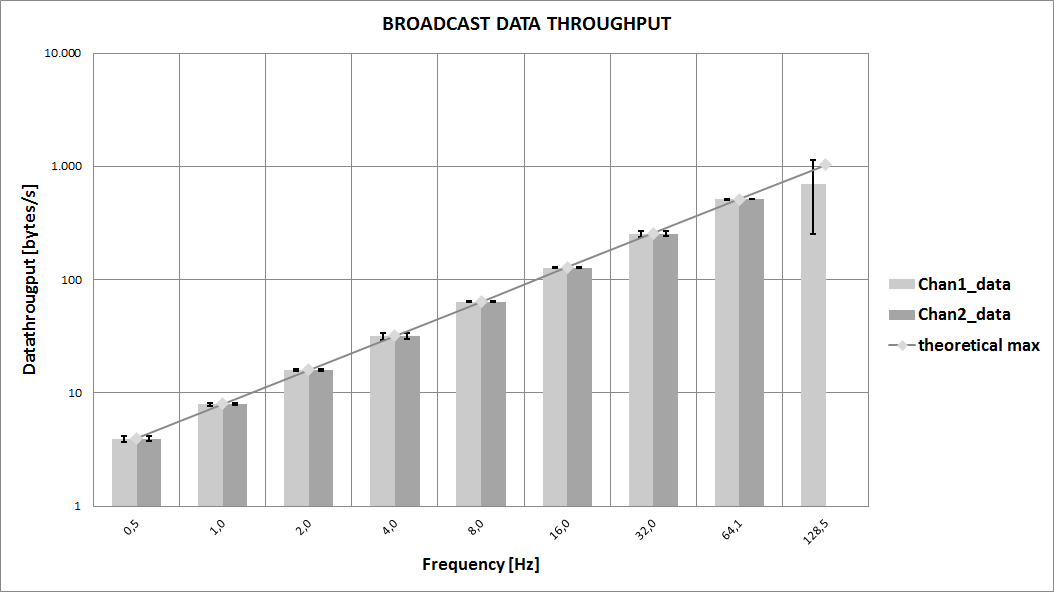
\includegraphics[scale=0.5]{content/images/exp2_norm.png}
		\caption{Broadcast data throughput - 2 channels (0.5Hz - 128.5Hz)}\label{fig:exp2low}
	\end{figure}
	Figures \ref{fig:exp2low} shows the results of the measurements, the left bar displaying the throughput for channel 1, the right bar displaying the throughput for channel 2. Just as in experiment 1 the  line shows the theoretical maximum of the data throughput for the given frequency. Up to a frequency of 64 Hz the data throughput increases with the frequency for both channels and matches the maximum value very closely. However the data throughput of channel 2  drops to zero at 128 Hz, while the data throughput of channel 1 almost matches the expected value, although the standard deviation indicates performance problems in this channel as well.
		\begin{figure}[H]
			\centering
			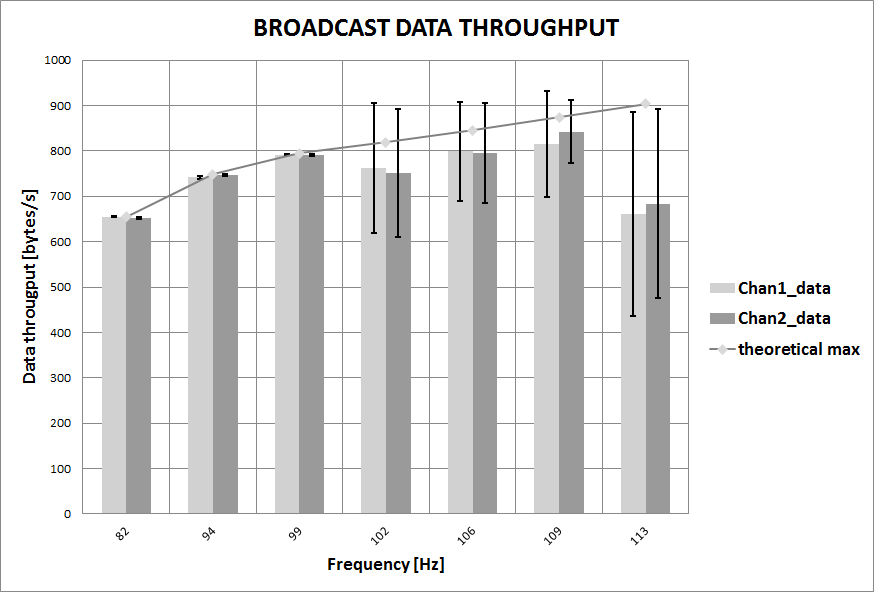
\includegraphics[scale=0.5]{content/images/exp2_detail.png}
			\caption{Broadcast data throughput - 2 channels (82Hz - 113Hz)}\label{fig:exp2high}
		\end{figure}
	To further investigate this drop off, figure \ref{fig:exp2high} shows the data throughput for chosen frequencies between 82 Hz and 113 Hz. Up to a frequency of 99 Hz the data throughput matches the expected values. For frequencies over 100 Hz however the data throughput drops off, while the measured errors increase. From this result we conclude two things: The 200 Hz capacity of the ANT chip is split between all channels the chip opened. In the test set up each chip can broadcast and receive with 100 Hz each, resulting in a data throughput of around 800 Bps for each channel. 	
\end{description}
\newpage


\section{Experiment 3: Acknowledge Data Transfer between two nodes}
\begin{description} 
	\item{\textbf{Description}} \hfill \\ This experiment is almost identical with experiment 1. The main difference is that we use acknowledge data instead of broadcast. It is also important to note that the master records how many successful packets are transmitted. The main goal of the experiment is to see whether the data throughput is decreased compared to broadcast data, especially for smaller channel periods.
	\item{\textbf{Use-Case}} \hfill \\ Scheduled data-transmission
	\item{\textbf{Network topology and pseudo code}} \hfill \\
	\begin{figure}[H]
		\centering
		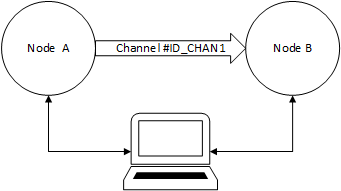
\includegraphics[scale=1]{content/images/exp_topo.png}
		\caption{Topology experiment 3}
	\end{figure}
	\begin{code}[H]
		\begin{verbatim}
		channelPeriod = max_Channel_Period
		while (channelPeriod >= min_Channel_Period) 
		  ANT_SetChannelPeriod(ID_CHAN1, channelPeriod)
		  ANT_OpenChannel(ID_CHAN1, ANT_Bidirectional_Master)
		  count = 0, fail = 0
		  for (10 seconds) 
		    ANT_SendAcknowledgedData(ID_CHAN1, [0x70, 0x69, 0x6E, 0x67])		    
		    if (receivedPacket() == ANT_ACKNOWLEDGED_DATA)		        
		      count++;			  
		    else if (receivedPacket() == ANT_MESSAGE_EVENT_RX_FAIL)
		      fail++;		    
		  print (count * 8 / 10) + " Bytes per second"	  
		  print fail + " failed transmissions
		  ANT_CloseChannel(ID_CHAN1)
		  if (channelPeriod >= 0x00FF)
		    channelPeriod = channelPeriod >> 1
		  else
		    channelPeriod = channelPeriod - 10
		\end{verbatim}
		\caption{Acknowledge data transfer (Master)}\label{lst:mExp3}
	\end{code}
	
	\begin{code}[H]
		\begin{verbatim}
		channelPeriod = max_Channel_Period
		while (channelPeriod >= min_Channel_Period) 
		  ANT_SetChannelPeriod(ID_CHAN1, channelPeriod)
		  ANT_OpenChannel(ID_CHAN1, ANT_Bidirectional_Slave)
		  wait_for_user_input()
		  ANT_CloseChannel(ID_CHAN1)
		  if (channelPeriod >= 0x00FF)
		    channelPeriod = channelPeriod >> 1
		  else
		    channelPeriod = channelPeriod - 10
		\end{verbatim}
		\caption{Acknowledge data transfer (Slave)}\label{lst:sExp3}
	\end{code}
	\item{\textbf{Testing methodology}} \hfill \\ The testing methodology is the same as in experiment 1, except that the master sends acknowledge messages and waits for the slave to confirm the successful transmission before sending the next packet. 
	\newpage
	\item{\textbf{Result}} \hfill \\
	\begin{figure}[H]
		\centering
		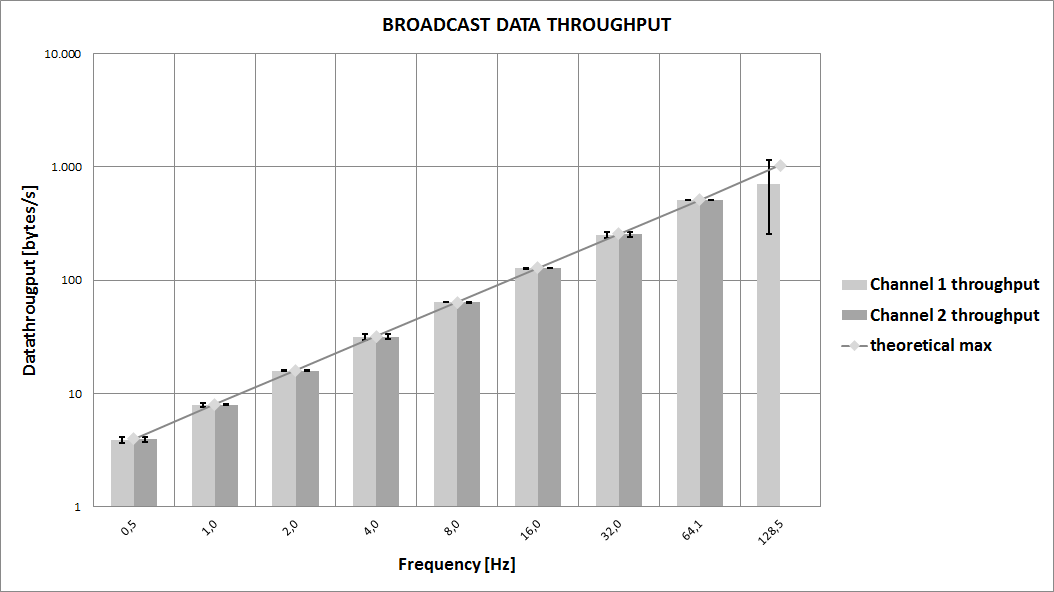
\includegraphics[scale=0.5]{content/images/exp3_norm.png}
		\caption{Acknowledge data throughput (0.5Hz - 128.5Hz)}\label{fig:exp4norm}
	\end{figure}
	\begin{figure}[H]
		\centering
		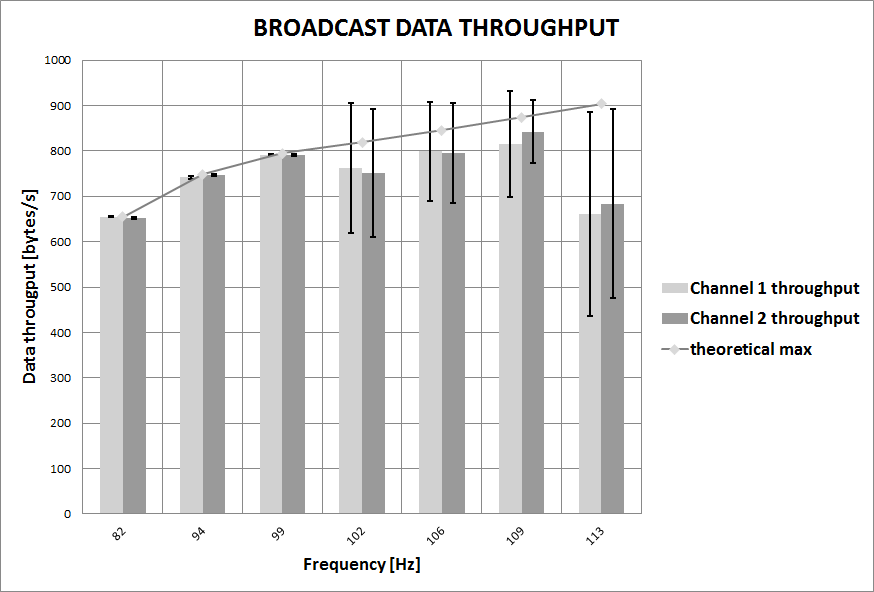
\includegraphics[scale=0.5]{content/images/exp3_detail.png}
		\caption{Acknowledge data throughput (65.4Hz - 69.6Hz)}\label{fig:exp4between}
	\end{figure}
	
	Figure \ref{fig:exp4norm} shows the measured transmission speeds for the different tested frequencies. For the lower frequencies the values align very well with the maximum theoretical data throughput. However, the tranmisson breaks down at 129 Hz. Figure \ref{fig:exp4between} shows the data throughput for some values between 65 Hz and 70 Hz, demonstrating that a drop off can be observed at around 69 Hz. 
	
	Since there is no increase of the data throughput above 68 Hz, but a huge drop off to about 50\% of the maximum theoretical throughput at higher frequencies and eventually a complete break down, the maximum data throughput for acknowledge data-transmissions is approximately 550 Bps.
\end{description}
\newpage

\section{Experiment 4: Acknowledge Data Transfer delay}
\begin{description} 
	\item{\textbf{Description}} \hfill \\ In this experiment we try to determine the time it takes for a node to receive and acknowledge a transmitted packet. The value is important in order to be able to determine the reaction time of SHAMPU to commands sent by the base station, for example to set up a separate channel for a burst transmission.
	\item{\textbf{Use-Case}} \hfill \\ Scheduled data-transmission
	\item{\textbf{Network topology and pseudo code}} \hfill \\ 
	\begin{figure}[H]
		\centering
		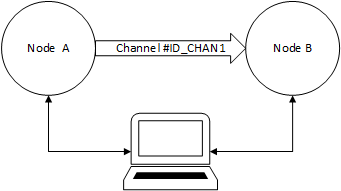
\includegraphics[scale=1]{content/images/exp_topo.png}
		\caption{Topology experiment 4}
	\end{figure}
	\begin{code}[H]
		\begin{verbatim}
		channelPeriod = max_Channel_Period
		while (channelPeriod >= min_Channel_Period) {
		  ANT_SetChannelPeriod(ID_CHAN1, channelPeriod)
		  ANT_OpenChannel(ID_CHAN1, ANT_Bidirectional_Master)
		  for (i in 0..10) {
		    ANT_SendAcknowledgedData(ID_CHAN1, [0x70, 0x69, 0x6E, 0x67])
		    start = getTime()	   
		    wait_for_ack()		
		    print (getTime() - start) + " s"	  
		  ANT_CloseChannel(ID_CHAN1)		
		  if (channelPeriod >= 0x00FF)
		    channelPeriod = channelPeriod >> 1
		  else
		    channelPeriod = channelPeriod - 10
		\end{verbatim}
		\caption{Acknowledge data delay (Master)}\label{lst:mExp4}
	\end{code}
	
	\begin{code}[H]
		\begin{verbatim}
		channelPeriod = max_Channel_Period
		while (channelPeriod >= min_Channel_Period)
		  ANT_SetChannelPeriod(ID_CHAN1, channelPeriod)
		  ANT_OpenChannel(ID_CHAN1, ANT_Bidirectional_Slave)
		  wait_for_user_input()
		  ANT_CloseChannel(ID_CHAN1)
		  if (channelPeriod >= 0x00FF)
		    channelPeriod = channelPeriod >> 1
		  else
		    channelPeriod = channelPeriod - 10
		\end{verbatim}
		\caption{Acknowledge data delay (Slave)}\label{lst:sExp4}
	\end{code}
	
	\item{\textbf{Testing methodology}} \hfill \\ Node A acts as the master and node B as the slave. For both nodes the channel period is set to the highest value and the channel is opened. Node A then sends a total of 10 acknowledge messages and measures how long it takes until it receives the
	acknowledge signal. The channel period is then decreased and the experiment repeated.
	
	\newpage
	\item{\textbf{Result}} \hfill \\  
	\begin{figure}[H]
		\centering
		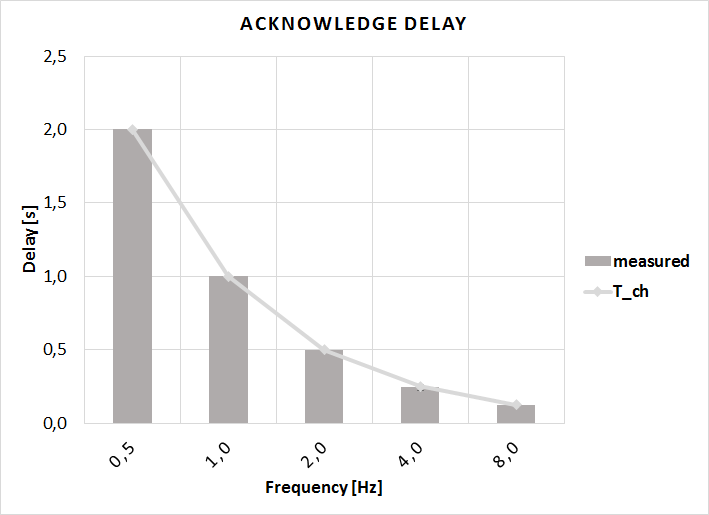
\includegraphics[scale=0.5]{content/images/exp4_norm.png}
		\caption{Acknowledge delay (0.5Hz - 8Hz)}\label{fig:exp3low}
	\end{figure}
	\begin{figure}[H]
		\centering
		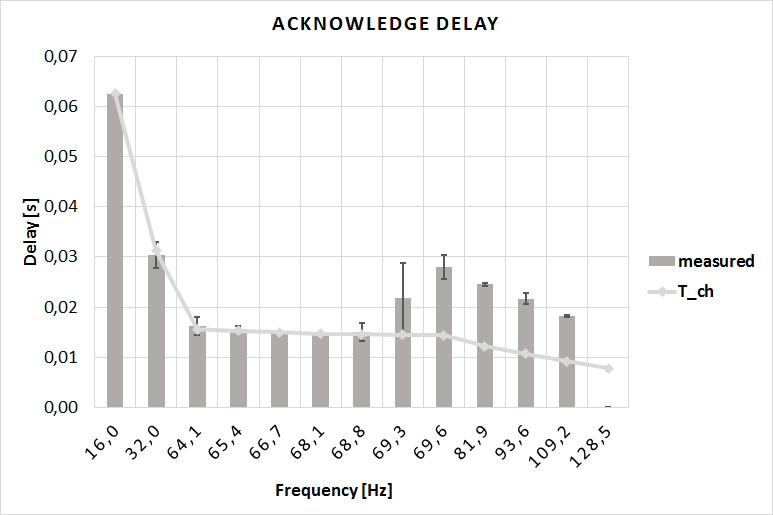
\includegraphics[scale=0.5]{content/images/exp4_detail.png}
		\caption{Acknowledge delay (16Hz - 128.5Hz)}\label{fig:exp3high}
	\end{figure}
	Figure \ref{fig:exp3low} and \ref{fig:exp3high} show the delays for the tested frequencies. The lines show the time $T_{ch}$ between two timeslots for various frequencies $f$, where $T_{ch} = \frac{1}{f}$. These values are in line with the measured delays until a frequency of 68.8Hz. 69.3 Hz represents a transition area, where the individual data points show delays with a duration of either one or two times $T_{ch}$. This explains the increased standard deviation. Above that frequency the delay corresponds with $2T_{ch}$ up to a frequency of at least 109 Hz. At 129 Hz no delay could be measured, as no acknowledge messages were correctly received. 

	We conclude, that in the given setup ANT requires at least 15 ms (equivalent to a frequency of 68.1 Hz) to confirm that a message has been successfully transmitted. If the time between the timeslots is shorter, it takes an additional timeslot to confirm the message. Due to lack of information about ANT, we cannot provide an explanation for this behaviour. Similarly we cannot offer a reason, why the acknowledge data-transmission breaks down completely at 128 Hz. The fact of the minimum delay of 15 ms explains why the maximum data throughput of acknowledge data is only 550 Bps.

\end{description}
\newpage

\section{Experiment 5: Burst Data Transfer between two nodes}
\begin{description} 
	\item{\textbf{Description}} \hfill \\ Burst data transmissions make it possible to drastically increase the throughput rate. This allows a SHAMPU base station to quickly transmit a new firmware to a node or a node to dump its RAM back to the base station.	According to the specification rates up to 20 kbps can be achieved. To fully utilize this speed a baud rate of 50000 is needed\cite{BurstMax}. In the current setup the base station uses 19200 baud, since it is the only value that both the ANT chip and the RS-232 interface support. Because of this we expect the maximum speed to be less than 20 kbps. Furthermore we try to determine whether the size of the burst transfer has an impact on the speed, since longer bursts will disrupt communications on other channels.
	\item{\textbf{Use-Case}} \hfill \\ Unscheduled data-transmission
	\item{\textbf{Network topology and pseudo code}} \hfill \\ 
	\begin{figure}[H]
		\centering
		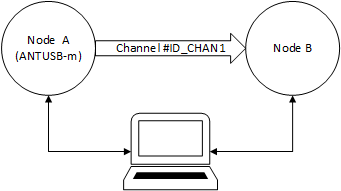
\includegraphics[scale=1]{content/images/exp5_topo.png}
		\caption{Topology experiment 5}
	\end{figure}
	\begin{code}[H]
		\begin{verbatim}
		size = 16
		ANT_OpenChannel(ID_CHAN1, ANT_Bidirectional_Slave);		
		while (size >= 16384)
		  for (i in 0..10) 
		    // The first packet of a burst has the 3 MSB of the channelID field set to 0
		    wait_until(received_Packet == ANT_BURST_DATA && 
		               (received_message_channelID[0] & 0xE0) == 0x00)
		    start = getTime()
		    // The last packet of a burst has the MSB of the channelID field set to 1
		    wait_until(received_Packet == ANT_BURST_DATA && 
		               (received_message_channelID[0] & 0x80) > 0)		    
		  print (size - 1) / (getTime() - start) " Bytes per second"
		  size *= 2
		\end{verbatim}
		\caption{Burst data transfer (Slave)}\label{lst:sExp5}
	\end{code}
	\item{\textbf{Testing methodology}} \hfill \\ Since the burst transmission mode of our ANT-library is not working correctly (see section \ref{sec:future}) we use an ANTUSB-m Stick, which acts as a master. Node B is a normal base station and receives the burst transfers. On the master side, the program ANTWareII \cite{ANTwareII} is used to create the channel and then send bursts with different sizes. Each size is sent 10 times and the values are recorded and averaged. The size is then doubled and the experiment repeated. The first burst packet cannot be counted directly since the start of the burst can only be determined after the ANT chip has already received the first packet.
	\newpage
	\item{\textbf{Result}} \hfill \\ 
	\begin{figure}[H]
		\centering
		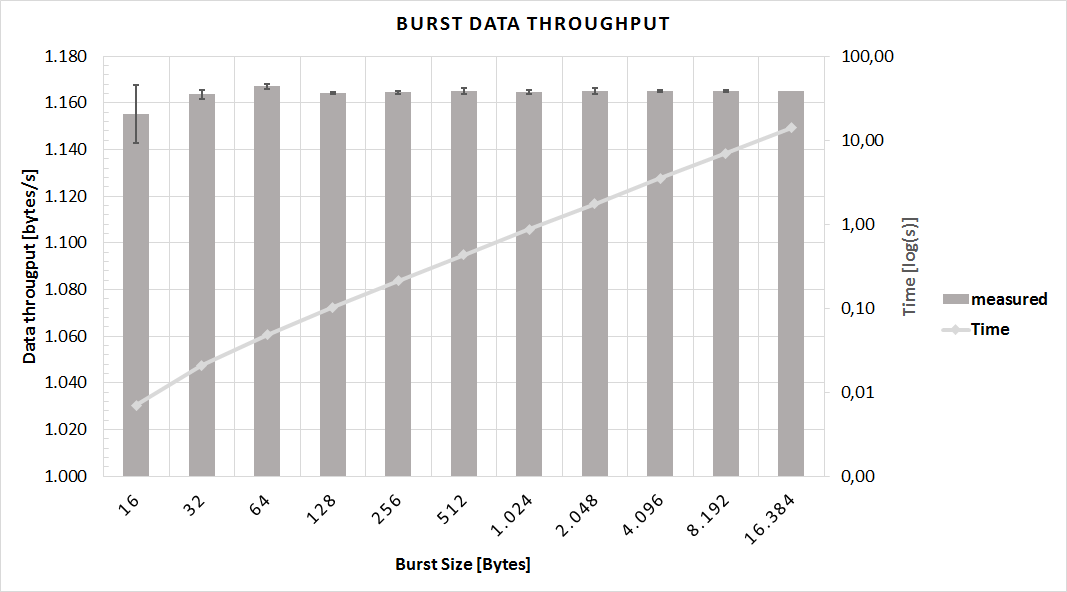
\includegraphics[scale=0.5]{content/images/exp5.png}
		\caption{Burst data throughput}\label{fig:exp5}
	\end{figure}
	Figure \ref{fig:exp5} shows the measured data throughput for the different packet sizes and also the length of the transfer. The values all hover around the same value of ~1165 Bps. This is approximately the same value as the one which can be achieved with the other two types of data.
	Again see section \ref{sec:dataThrougput} for a discussion about possible reasons for this upper limit. 
\end{description}
\newpage

\section{Experiment 6: Maximum communication range}
\begin{description} 
	\item{\textbf{Description}} \hfill \\  In this experiment we try to determine the correlation between the maximum range and the power setting of the ANT radio. One of SHAMPU's advantages is the low power consumption. It might be possible to further reduce the power consumption by decreasing the power level of the ANT radio, especially in smaller environments where there is no need for a long range. According to the datasheet the maximum range for communication is 30m, however the ANT documentation does not provide different ranges for different power settings. 
	
	\item{\textbf{Use-Case}} \hfill \\ Unscheduled data-transmission and scheduled data-transmission	
	\item{\textbf{Network topology and pseudo code}} \hfill \\ 
	\begin{figure}[H]
		\centering
		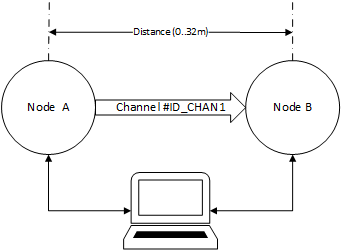
\includegraphics[scale=1]{content/images/exp6_topo.png}
		\caption{Topology experiment 6}
	\end{figure}
	
	\begin{code}[H]
		\begin{verbatim}
		for (pSetting in Available_PowerSettings)
		  ANT_SetTransmitPower(pSetting)
		  openChannel(ID_CHAN1, ANT_Bidirectional_Master)
		  ANT_SendBroadcastData(ID_CHAN1, [0x70, 0x69, 0x6E, 0x67])
		  wait_for_user_input()
		  closeChannel(ID_CHAN1)
		\end{verbatim}
		\caption{Maximum communication range (Master)}\label{lst:mExp6}
	\end{code}
	
	\begin{code}[H]
		\begin{verbatim}
		distance = 0.0
		stopInc = false
		loop 
		  openChannel(ID_CHAN1, ANT_Bidirectional_Slave)
		  wait_until(received_Packet == ANT_BROADCAST_DATA || 
		             received_Packet == ANT_MESSAGE_EVENT_RX_SEARCH_TIMEOUT) 
		  if (stopInc) 
		    if (wasTimeout) 
		      distance -= .4
		    else 
		      print "Connection found : " + distance
		  else
		    if (wasTimeout)  
		      stopInc = true
		      distance -= .4
		      print "Connections lost : " + distance
		    else distance += .4
		  closeChannel(ID_CHAN1)
		\end{verbatim}
		\caption{Maximum communication range (Slave)}\label{lst:sExp6}
	\end{code}
	\item{\textbf{Testing methodology}} \hfill \\ At the beginning of the experiment Node A and B are placed right next to each other. Node A acts as a master and keeps broadcasting the same message. Node B is the slave and tries to connect to the channel. If the connection is successful, the distance between the two nodes is increased by 0.4 meters. This process is repeated until Node B can no longer connect to the channel and the connection times out. This happens after 30s of searching. At this point the distance is no longer increased, but rather decreased until Node B is able to successfully connect to the channel. Both of these values are recorded and averaged. The whole experiment is then repeated for each available power setting.	
	\newpage
	\item{\textbf{Result}} \hfill \\ 
	\begin{figure}[H]
		\centering
		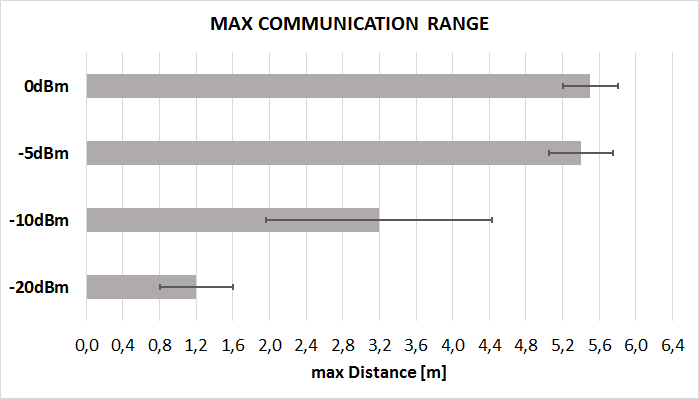
\includegraphics[scale=0.5]{content/images/exp6.png}
		\caption{Maximum communication range}\label{fig:exp6}
	\end{figure}
	Figure \ref{fig:exp6} shows the transmission range for each power setting. As expected the maximum distance goes up with the higher power settings. But the result at the highest power setting is disappointing, since we did not get close to the claimed maximum range of 30m. The ANT documentation states that the maximum range of 30m can only be achieved in "optimal conditions" \cite{DynastreamInnovationsInc.2013}. It is possible for several different unfavorable factors to interfere with the ANT signal, such as multiple 802.11 networks in the vicinity, or even the plastic case of the base station. 
\end{description}

\newpage
\section{Maximum Data Throughput}
\label{sec:dataThrougput}

In our experiments we were able to confirm two important limits for the maximum data throughput which can be achieved with our current setup. The ANT AP1MxIB supports a maximum message frequency of 200 Hz, which means that we would expect to see a maximum transmission rate of 1600 Bps.
However, this limit can only be achieved by splitting the available bandwidth between receiving and sending. If we try to utilize the full 200 Hz only for either receiving or sending, we are limited to 1100 Bps, around 500 Bps or 30\% lower than the theoretical maximum. A similar limit of 1165 Bps holds for burst transmissions, where we loose around 1335 Bps or 53\% of the maximum theoretical data throughput.\\

For acknowledge data, only a data throughput of 550 Bps could be achieved. The analysis of individual data points suggest, that the acknowledge reply consumes an additional time slot for frequencies above 69 Hz. At 128 Hz no successful data transmission could be confirmed.\\

To balance environmental influences, the experiments were repeated in different locations and times of day and night. Since the throughput did not change noticeably, it can be assumed that there are no easily eliminated environmental factors affecting the maximum rate. We conclude that the root cause for the lower than expected throughput must be attributed to the hardware or software. \\

If we exclude environmental factors, the limitations could be based on certain parts of the test setup:
\begin{itemize}
	\item{\textbf{RS-232 Connection}} \hfill \\ The base station is connected to a PC over a serial connection. For the speed we chose 19200 baud, since it is the highest value supported by the ANT chip and the serial-Interface. With 19200 baud the maximum data throughput of the RS-232 connection is 1920 Bps, since the interface adds a start and stop bit to each byte. If the serial connection would be the bottle neck for burst transmission, we would expect to get the full 1920 Bps of data throughput. Since this is not the case we can conclude that the RS-232 connection is not the limiting factor. This is supported by the similarity of the limits for broadcast and burst transmissions.

	\item{\textbf{ANT API}} \hfill \\ The software we use is not officially supported by ANT. It is thus possible that there are some bugs which have an impact on the performance. Except for the missing burst mode (see \ref{sec:future}), there were no unusual measured values during the experiments. If there is a bug, it might be hard to find without rewriting all the experiments and running them with the official ANT library \cite{ANTWinLib}
	
	\item{\textbf{ANT AP1MxIB}} \hfill \\ Due to the black box nature of ANT, it is very hard to exactly determine what might cause a performance deficit. The inner workings of the chip are not documented, and the error messages of the protocol are not very specific. The chip itself is from 2007 and the manufacturer no longer recommends the use of the chip\cite{AP1page}. There are alternatives available, like the newer ANTAP281M5IB chip \cite{AP2Datasheet}.
\end{itemize}
\newpage